\documentclass[english]{tktltiki}
\usepackage[pdftex]{graphicx}
\usepackage{subfigure}
\usepackage{url}
\usepackage{enumerate}
\usepackage{amsmath}
\usepackage{hyperref}
\begin{document}
\onehalfspacing

\title{Location Awareness - Week 4}
\author{P�ter Ivanics}
\date{\today}

\maketitle

\numberofpagesinformation{\numberofpages\ pages + \numberofappendixpages\ appendices}
\keywords{}

\mytableofcontents

\section{Concepts}
	\begin{enumerate}[a)]
		\item Velocity pruning is a type of pruning (reduction of non-meaningful measurement data), where positions, in between the user was moving with high speed are not considered as meaningful places. In other words, the only meaningful places of a measurement set are the areas, where user spends significant amount of time, ergo is not moving fast. Typically a velocity threshold is given to determine the meaningful points and therefore places. 
		
		The attached $velocity_pruning.R$ script performs simple pruning on the data. Figure \ref{velocity_pruning} displays the points before and after pruning. Looking at the original dataset on the left graph it is visible that the points seem to be scattered around two places. The movement speed can be easily estimated by calculating the distance between the points and dividing the distances by the elapsed time respectively. 
		
		The velocity threshold is set to the mode of the estimated velocities ($3.8$). This seems to be a good choice in this case as the mean and the median gives worse results. By redrawing the points that exceed this value it is visually visible, that two places can be clearly identified. There are still some standalone points outside these two areas but they can not be considered as meaningful places. 
		
		\begin{figure}[h] 
			\begin{center}
				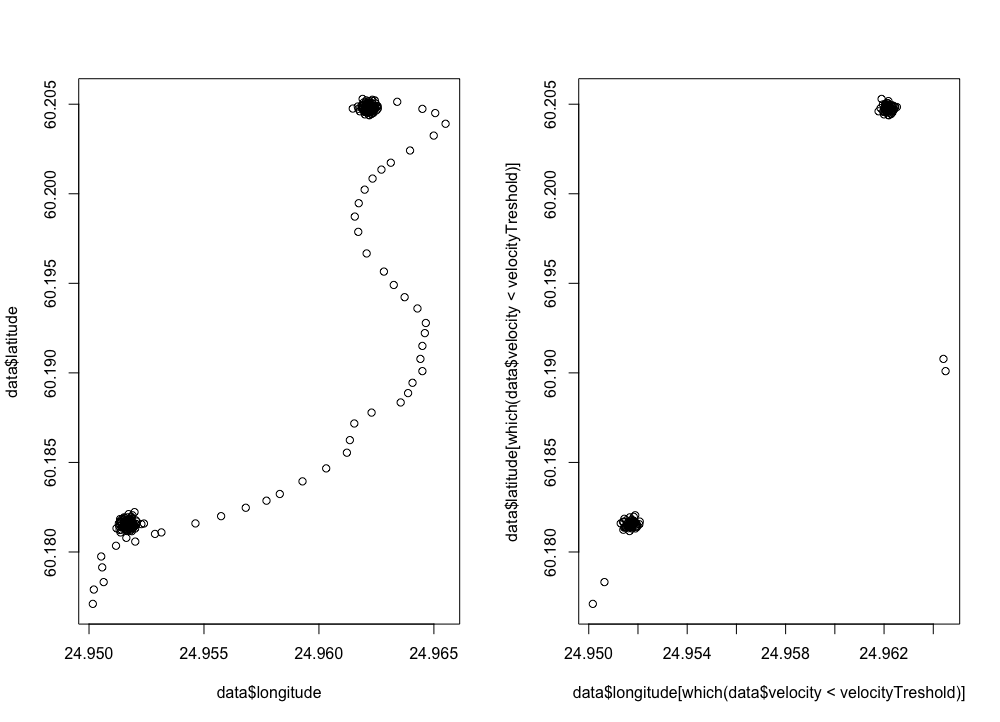
\includegraphics[width=0.75\textwidth]{images/velocity_pruning.png}
				\caption{The scatter plot of the points before (left) and after (right) the velocity pruning.}
				\label{velocity_pruning}
			\end{center}
		\end{figure}
	\item The $q$ value in the Markov chain refers to the order/memory of the model. The probability of state $x_k$ is given by the probability $p(x_k | x_{1:k-1})=p(x_k | x_{k-q-1:k-1})$	, where $x_k$ is the state of the system at time $k$, $q$ is the order of the model. In other words this means, to estimate the probability $k^{th}$ system state, $q$ number of previous observations observations are utilized. Accordingly, the first order Markov model relies only on the last two observations, while a model of the $q^{th}$ order would extend the estimations with previously collected data.
		
	\end{enumerate}

	

\section{Fingerprint-Based Place Detection}

\section{Lempel-Ziv}

\section{Spatial Analysis: Preprocessing and Place Detection}
	
\nocite{*}
\bibliographystyle{tktl}
\bibliography{lahteet}

\lastpage

\pagestyle{empty}

\end{document}